\section{Rとは}
\begin{wrapfigure}[7]{r}[2.5truemm]{40truemm}
\centering
\vspace{-2em}
\includegraphics[width=38truemm]{img/Rlogo.eps}
\vspace{-1em}
\end{wrapfigure}
1996年に登場した,オープンソースでフリーの統計解析向け言語及び開発実行環境であり,最新バージョンは2016/05/03にリリースされた 3.3.0 (Supposedly Educational).
Linux,Windows,OSX で利用可能である.
似た言語では S言語があり,Rが開発される前にAT\&Tベル研究所によって開発された統計処理言語である.

Rではさまざまな構造のデータを保持でき,記法がC言語に似ている為,習得が大変容易である.
コントリビュータによって用意されるパッケージも豊富で,その数は5000個以上である.

\section{Rをインストールしよう}
まず,{\tt http://www.r-project.org/} にアクセスし,左サイドバーの CRAN をクリックすると,CRAN のミラーサーバを選択する画面が表示されるので,なるべく日本のミラーサーバを選択する.
日本でのミラーサーバは山形大学・統計数理研究所に存在している.
オススメは統計数理研究所(Institute of Statistical Mathematics, Tokyo).

ミラーサーバにアクセスし,OSを選択する.
以下の作業は,リリースされている最新バージョンによって表示が多少異なる.
また,インストール時の画像は R3.0.2 のものである.

\subsection{Windowsの場合}
\underline{Download R for Windows} → \underline{base} → \underline{Download R 3.2.0 for Windows} (62 megabytes, 32/64 bit) の順にクリックし,インストーラをダウンロードする.

\includegraphics[width=2cm]{img/windows/win001.eps} ダウンロードしたインストーラを起動し,以下のダイアログを進めていく.

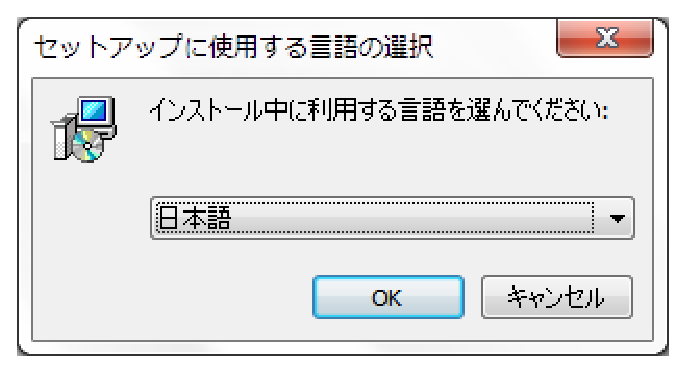
\includegraphics[width=6cm]{img/windows/win002.eps}\hspace{0.8em} 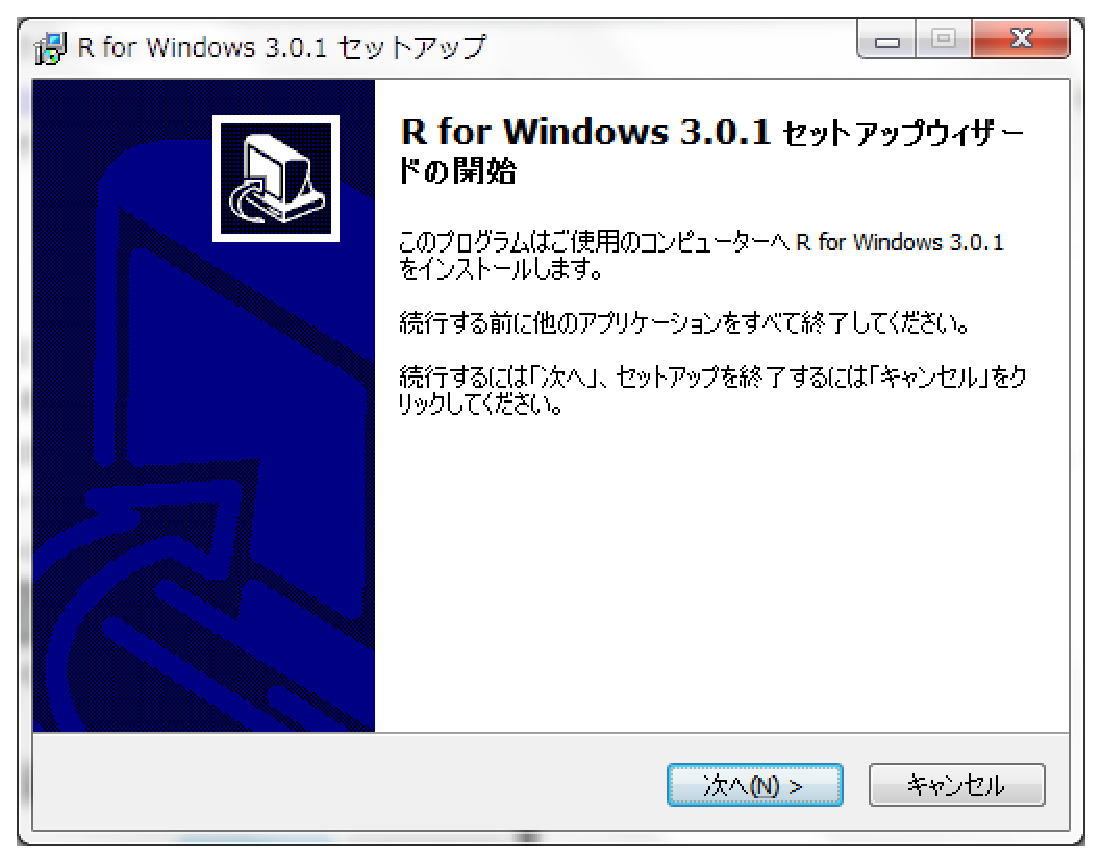
\includegraphics[width=8cm]{img/windows/win003.eps}\\

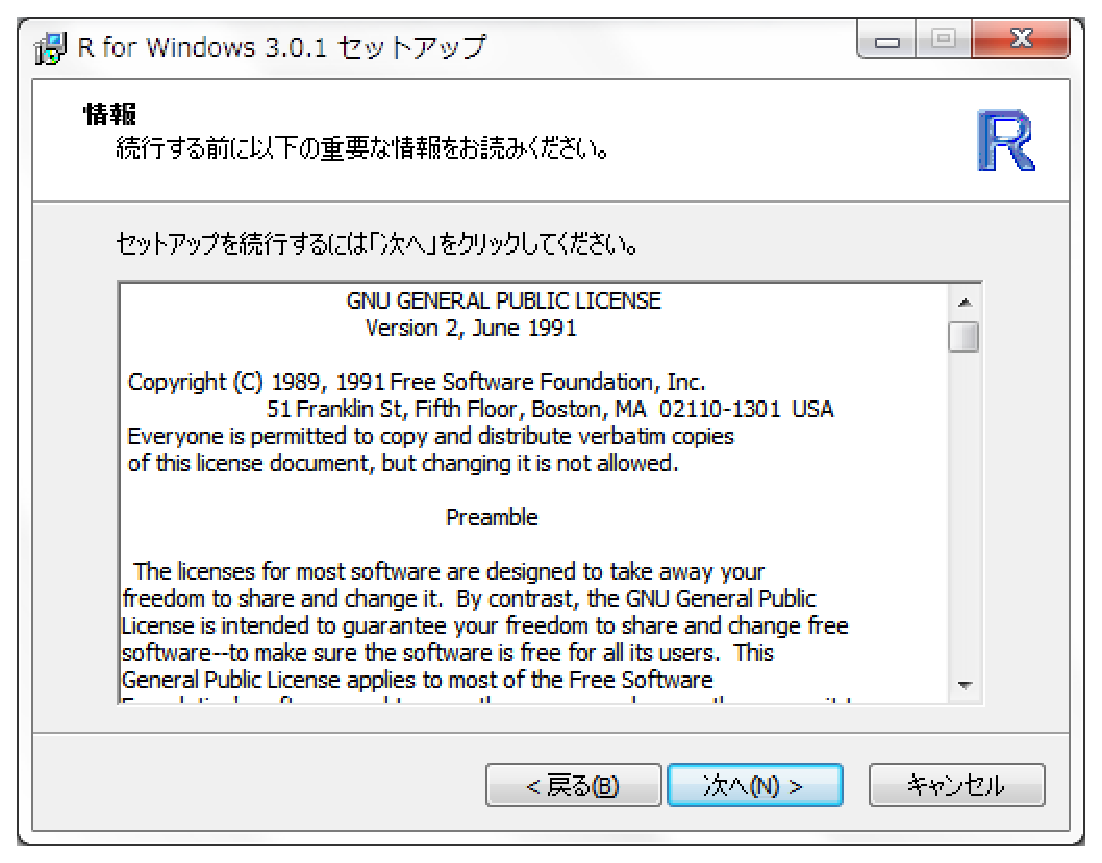
\includegraphics[width=8cm]{img/windows/win004.eps}\hspace{0.8em} 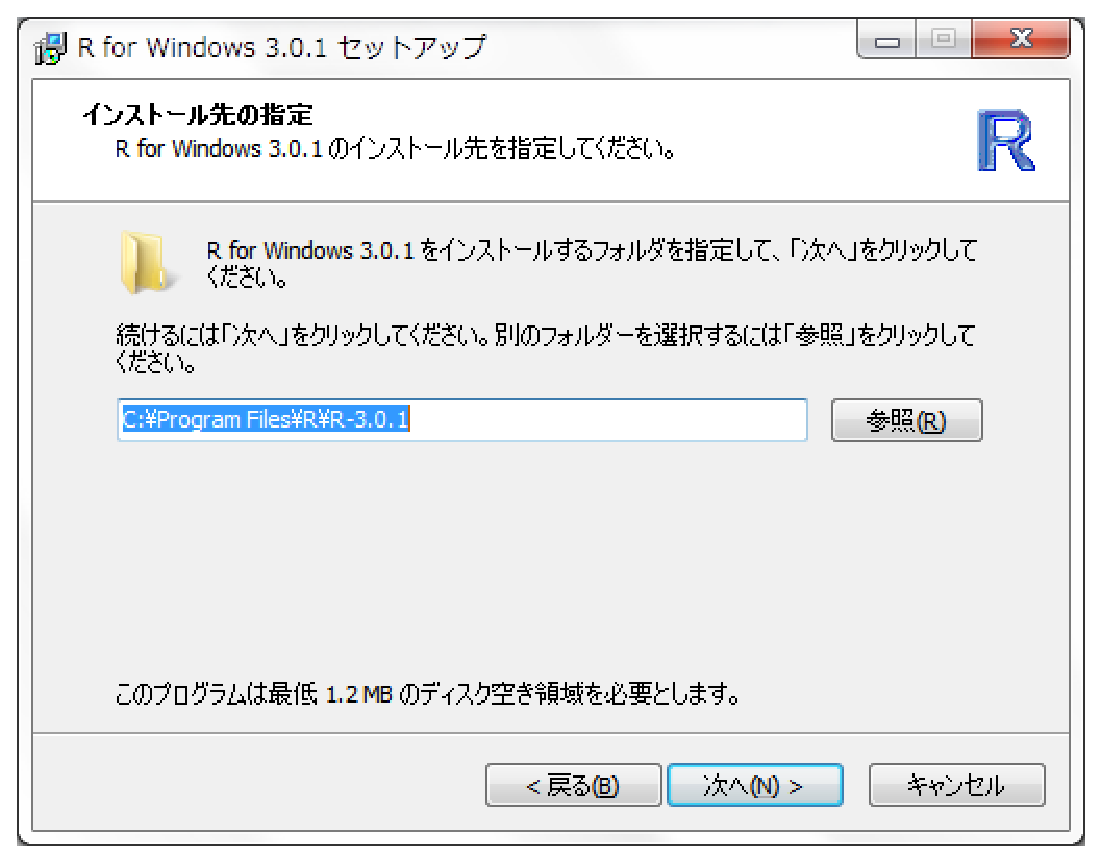
\includegraphics[width=8cm]{img/windows/win005.eps}\\

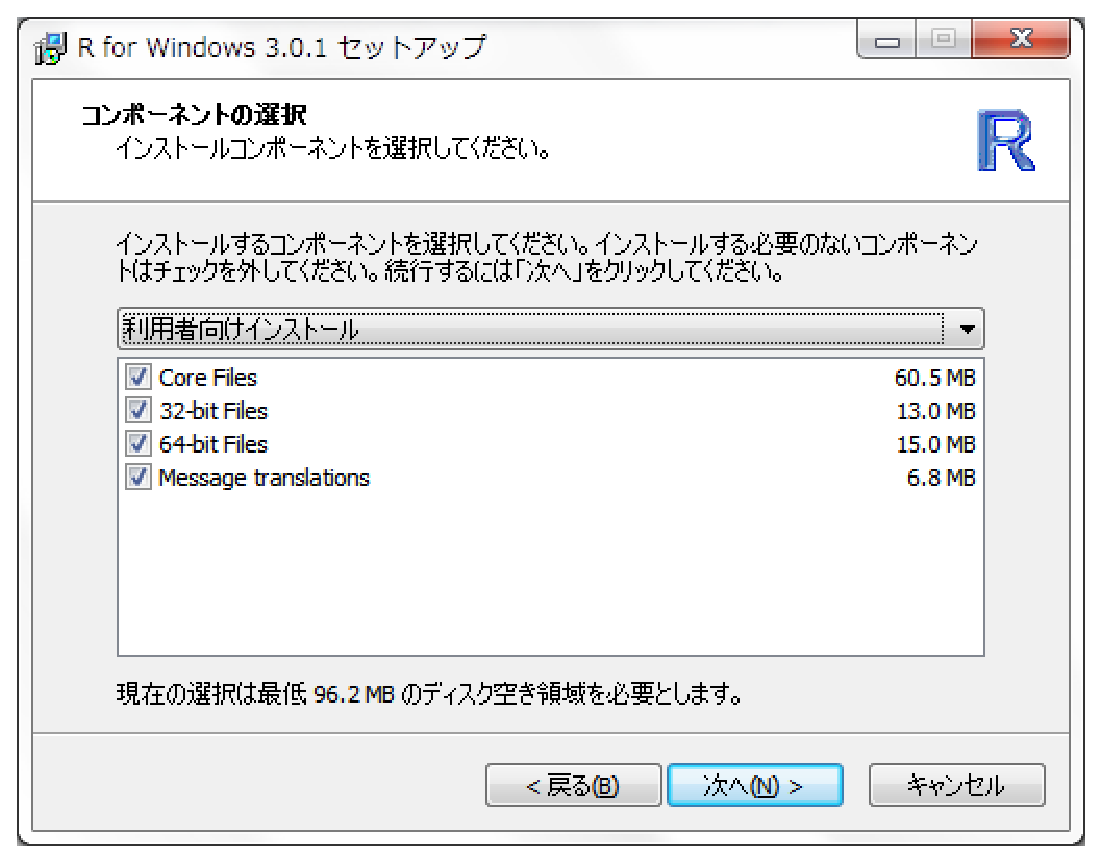
\includegraphics[width=8cm]{img/windows/win006.eps}\hspace{0.8em} 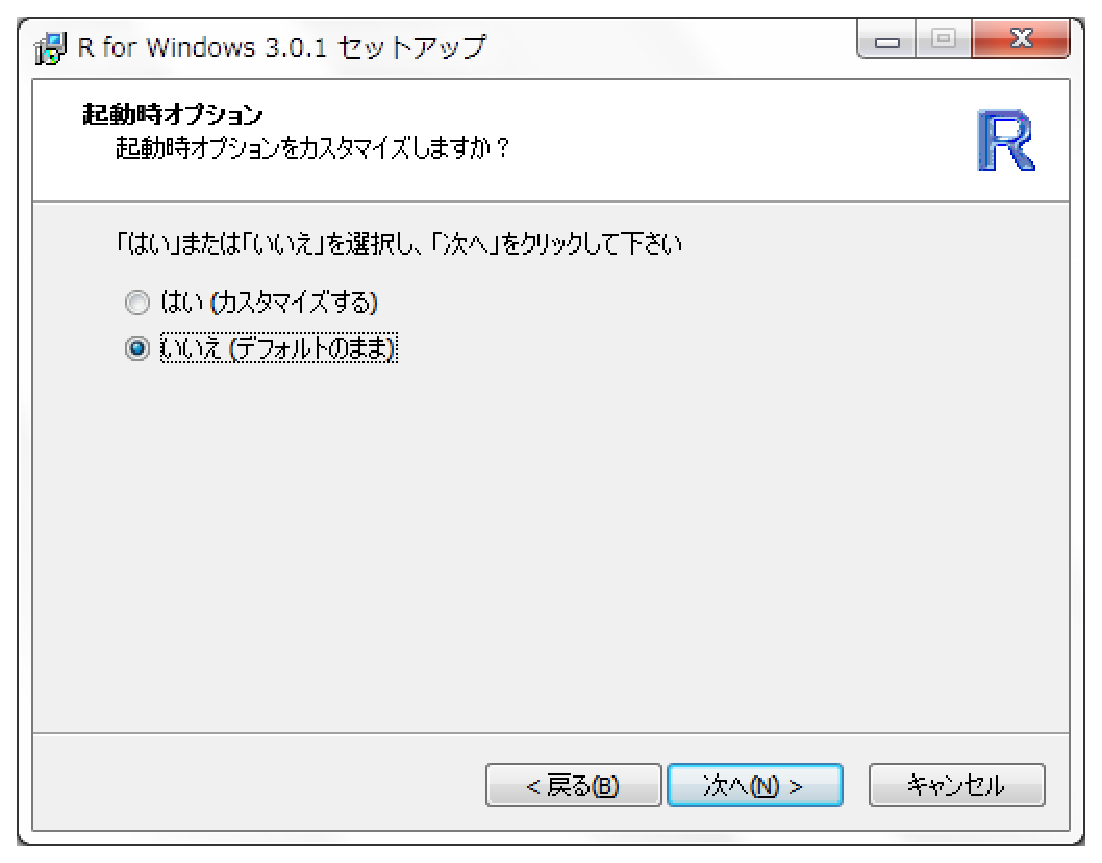
\includegraphics[width=8cm]{img/windows/win007.eps}\\

\includegraphics[width=8cm]{img/windows/win008.eps}\hspace{0.8em} 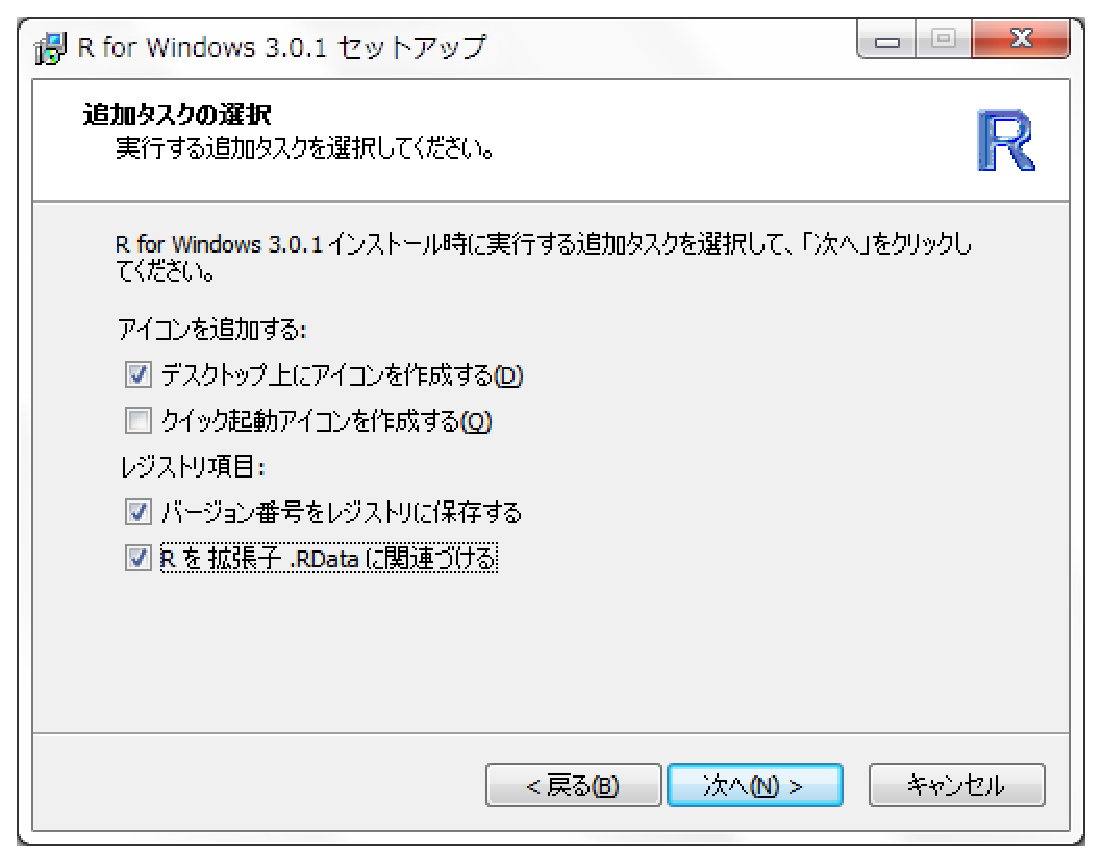
\includegraphics[width=8cm]{img/windows/win009.eps}\\

\includegraphics[width=8cm]{img/windows/win010.eps}\hspace{0.8em} 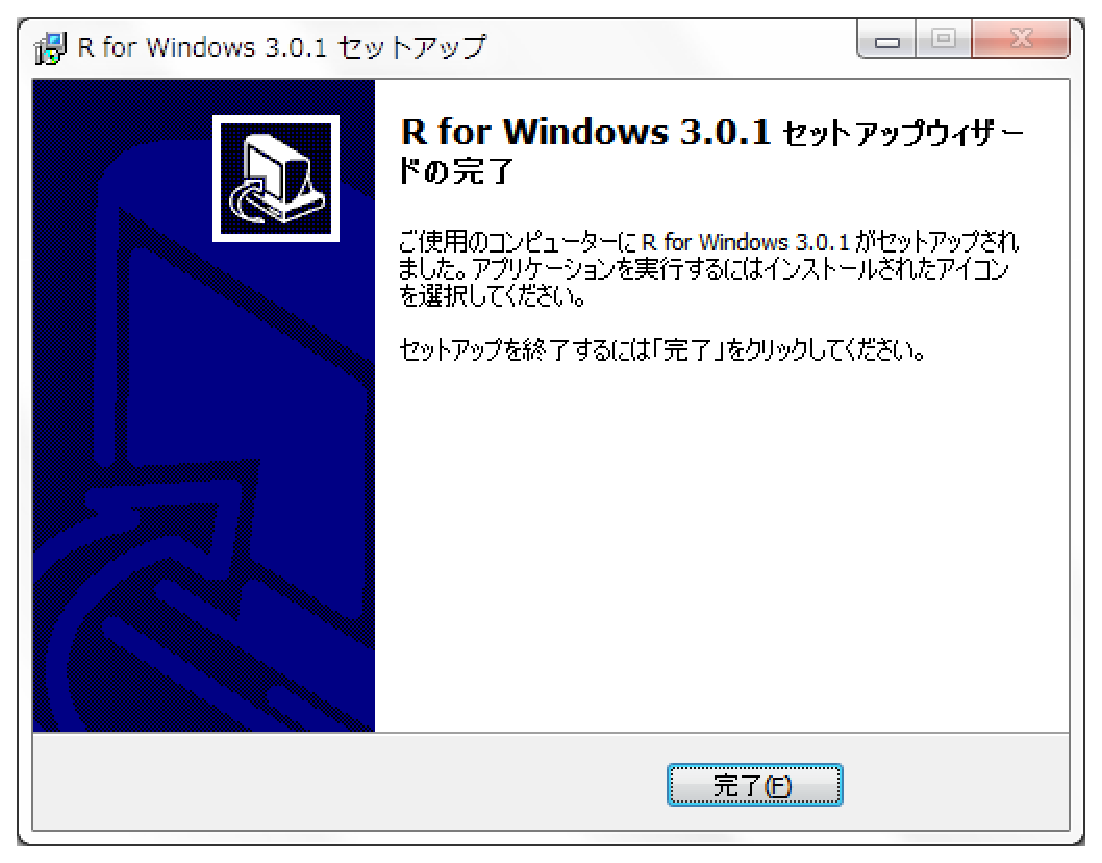
\includegraphics[width=8cm]{img/windows/win011.eps}\\

以上でインストールは完了する.\\

デスクトップに作成されたショートカット 
\includegraphics[width=1.7cm]{img/windows/win012.eps}より起動する.
\subsection{OSX (Mac)の場合}
\underline{Download R for (Mac) OS X} → \underline{R-3.2.0.pkg} の順にクリックし,インストーラをダウンロードする.\\
OS が古い場合は\underline{R-3.1.3-snowleopard.pkg}を用いてインストールする.

\includegraphics[width=1.8cm]{img/osx/osx001.eps} ダウンロードしたインストーラを起動し,以下のダイアログを進めていく.\\

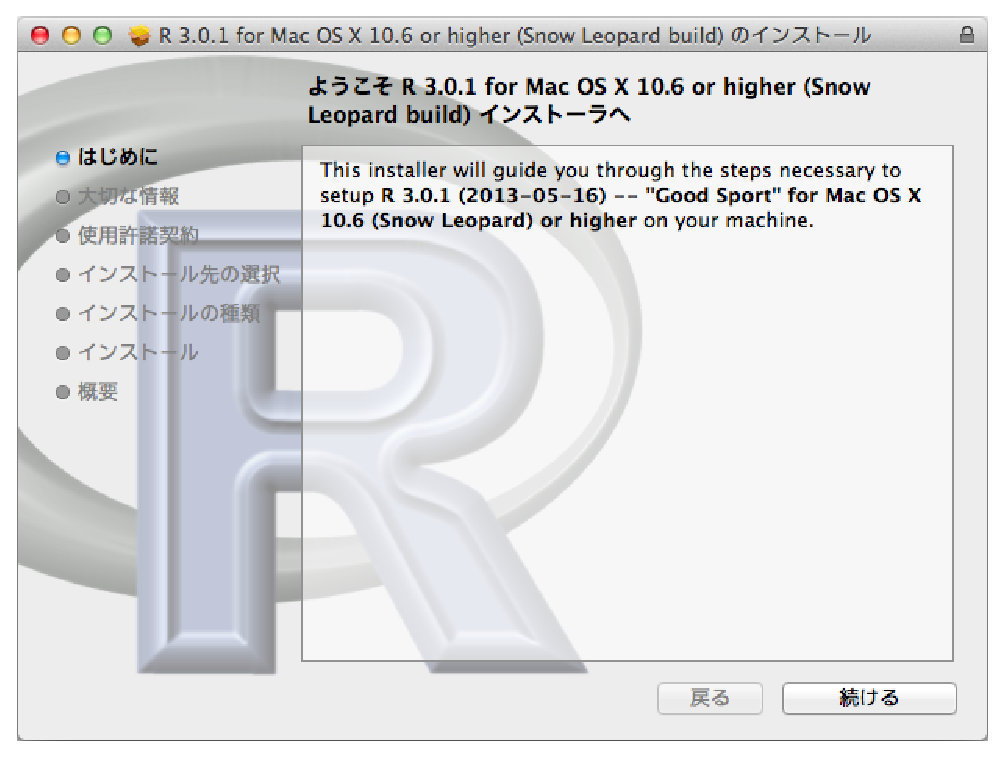
\includegraphics[width=8cm]{img/osx/osx002.eps}\hspace{0.8em} 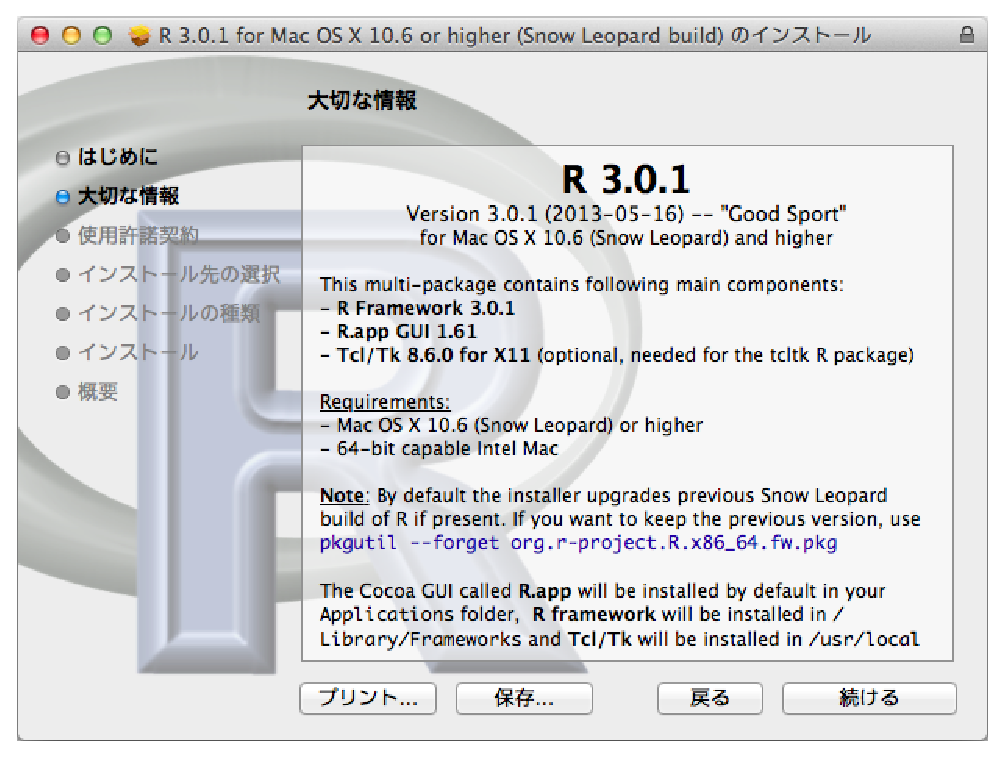
\includegraphics[width=8cm]{img/osx/osx003.eps} \\

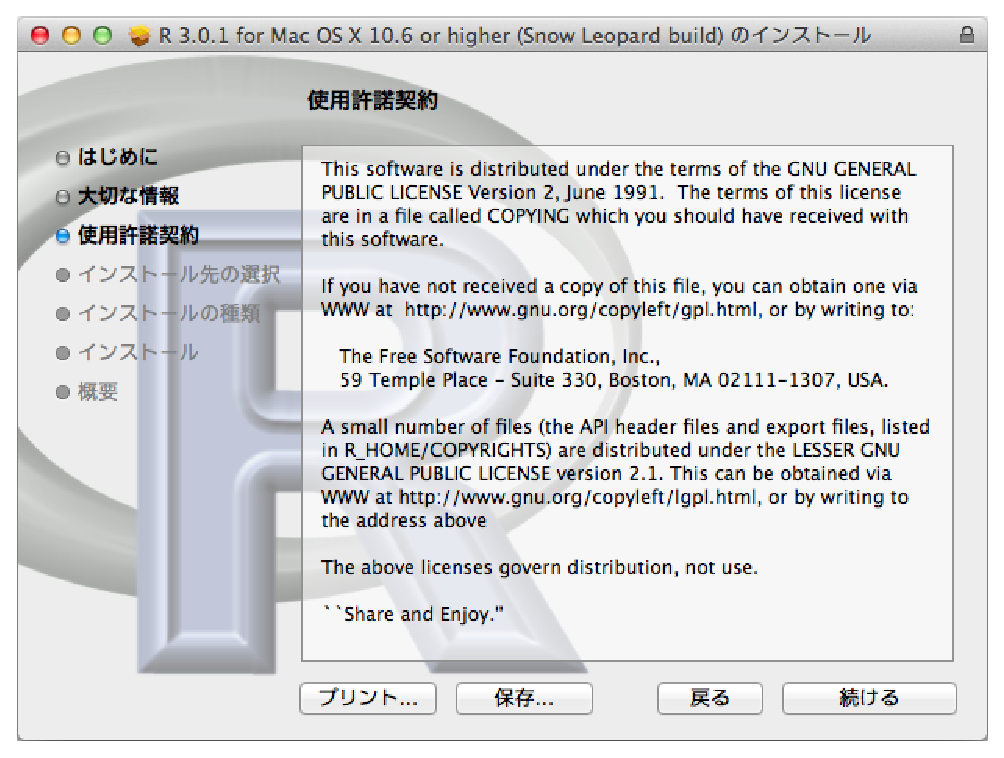
\includegraphics[width=8cm]{img/osx/osx004.eps}\hspace{0.8em} 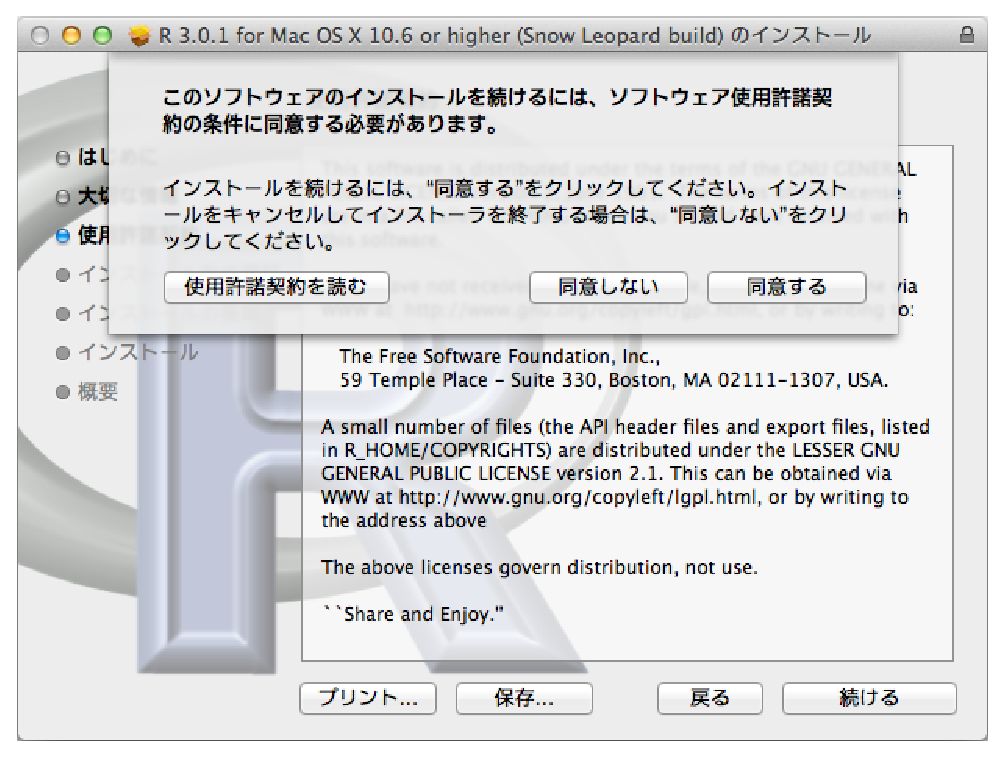
\includegraphics[width=8cm]{img/osx/osx005.eps}\\

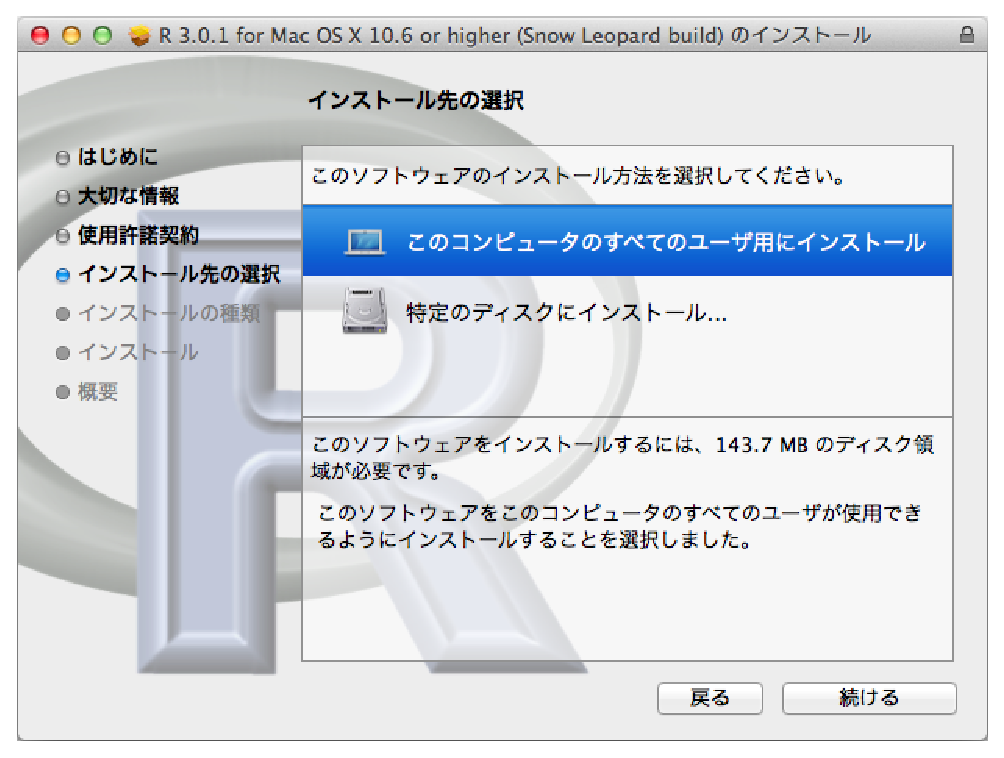
\includegraphics[width=8cm]{img/osx/osx006.eps}\hspace{0.8em} \includegraphics[width=8cm]{img/osx/osx007.eps}\\

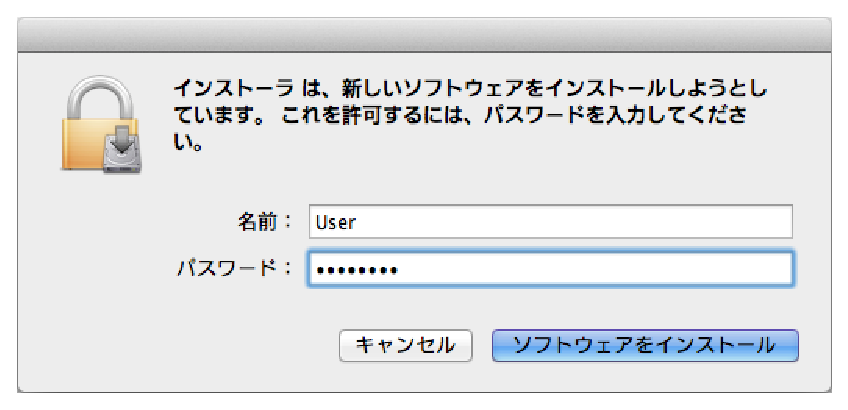
\includegraphics[width=8cm]{img/osx/osx008.eps}\hspace{0.8em} 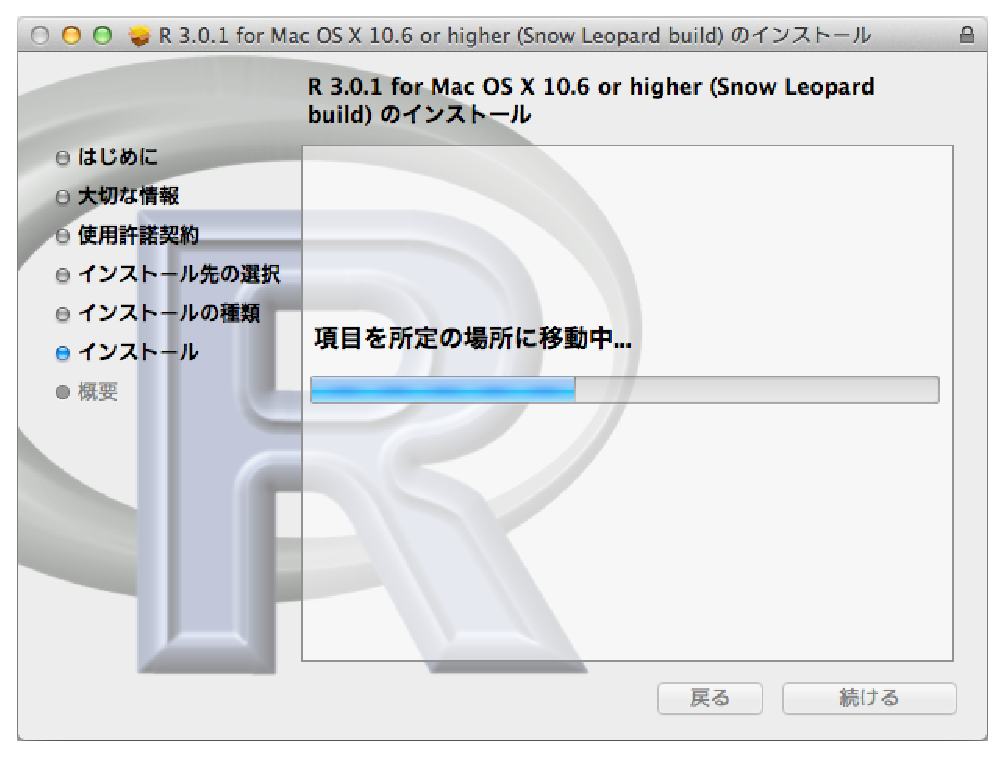
\includegraphics[width=8cm]{img/osx/osx009.eps}\\

\includegraphics[width=8cm]{img/osx/osx010.eps}\hspace{0.8em} \includegraphics[width=8cm]{img/osx/osx011.eps}\\

以上でインストールは完了する.\\

アプリケーションにある 
\includegraphics[width=1.8cm]{img/osx/osx012.eps}より起動する.
\subsection{Linuxの場合}
パッケージ管理システムでインストールが可能.\verb+apt-get+では以下の様にインストールを行う.
\begin{breakbox}
\begin{verbatim}
sudo apt-get update
sudo apt-get install r-base
\end{verbatim}
\end{breakbox}
しかしながら,最新版への更新は遅めになるので,以下のように設定しても良い.
\verb+/etc/apt/sources.list+を管理者権限でで編集し
\begin{breakbox}
\begin{verbatim}
deb http://cran.ism.ac.jp/bin/linux/ubuntu precise/
\end{verbatim}
\end{breakbox}
を最終行に追記.
\begin{breakbox}
\begin{verbatim}
gpg --keyserver keyserver.ubuntu.com --recv-key E084DAB9
gpg -a --export E084DAB9 | sudo apt-key add -
sudo apt-get update
sudo apt-get install r-base
\end{verbatim}
\end{breakbox}
r-baseのレポジトリが標準のubuntuミラーではなくなりCRANのものになる.\\
細かい話は \url{http://www.trifields.jp/install-r-in-ubuntu-1000} や\\ \url{http://www.trifields.jp/how-to-deal-with-when-you-can-not-update-the-r-in-ubuntu-1515} あたりを参照してください.